\chapter{p-ब्लॉक I: बोरॉन, कार्बन और नाइट्रोजन समूह}\label{ch:b1:p-block-13-15}

जिस वायु में हम साँस लेते हैं उसका चार-पाँचवाँ भाग नाइट्रोजन है, फिर भी पौधे उसके लिए भूखे रहते हैं:
\ce{N#N} त्रि-आबंध इतना प्रबल है कि लगभग कुछ भी उसे नहीं तोड़ता। इतिहास के अधिकांश
समय में फ़सलों का नाइट्रोजन खाद से, फलीदार पौधों की जड़ों पर रहने वाले
जीवाणुओं से, और खोदे गए नाइट्रेटों से आता था। बीसवीं शताब्दी के आरंभ में
लोहे के \omterm{def:b1:elementary-steps:catalyst}{उत्प्रेरक} पर नाइट्रोजन और हाइड्रोजन के बीच एक अभिक्रिया ने
इसे बदल दिया; आज संसार प्रति वर्ष अमोनिया के रूप में लगभग 16 करोड़ टन नाइट्रोजन
बनाता है, और मानव शरीर के नाइट्रोजन का लगभग आधा भाग किसी
अमोनिया संयंत्र से होकर गुज़रा है। \omterm{def:b1:periodicity:table}{समूह} 13, 14 और 15 में उस कहानी के तत्त्व हैं
--- उर्वरकों के लिए नाइट्रोजन और फ़ॉस्फ़ोरस, जीवन और चट्टानों के लिए कार्बन और
सिलिकॉन, काँच और हल्की मिश्रधातुओं के लिए बोरॉन और ऐलुमिनियम। यह
अध्याय पिछले अध्यायों के उपकरणों से उनका सर्वेक्षण करता है।

\begin{recall}
कार्बन के \omterm{def:b1:crystals-metals:allotropy}{अपररूप} तथा सिलिकॉन और सिलिका की संरचना
(\cref{ch:b1:crystals-ionic-covalent}); ऑक्साइडों का स्वभाव
(\cref{def:b1:s-block:oxide-character}); \omterm{def:b1:nernst:oxidation-number}{ऑक्सीकरण संख्याएँ} और \omterm{def:b1:nernst:electrode-potential}{मानक
विभव} (\cref{ch:b1:nernst}); \omterm{def:b1:precipitation:amphoteric-hydroxide}{उभयधर्मी हाइड्रॉक्साइड}
(\cref{ch:b1:precipitation}); गिब्ज़ ऊर्जाओं से साम्य स्थिरांक
(\cref{ch:b1:extent-q-and-k})।
\end{recall}
% ledger: usgs:N-world-2025

\begin{omfigure}
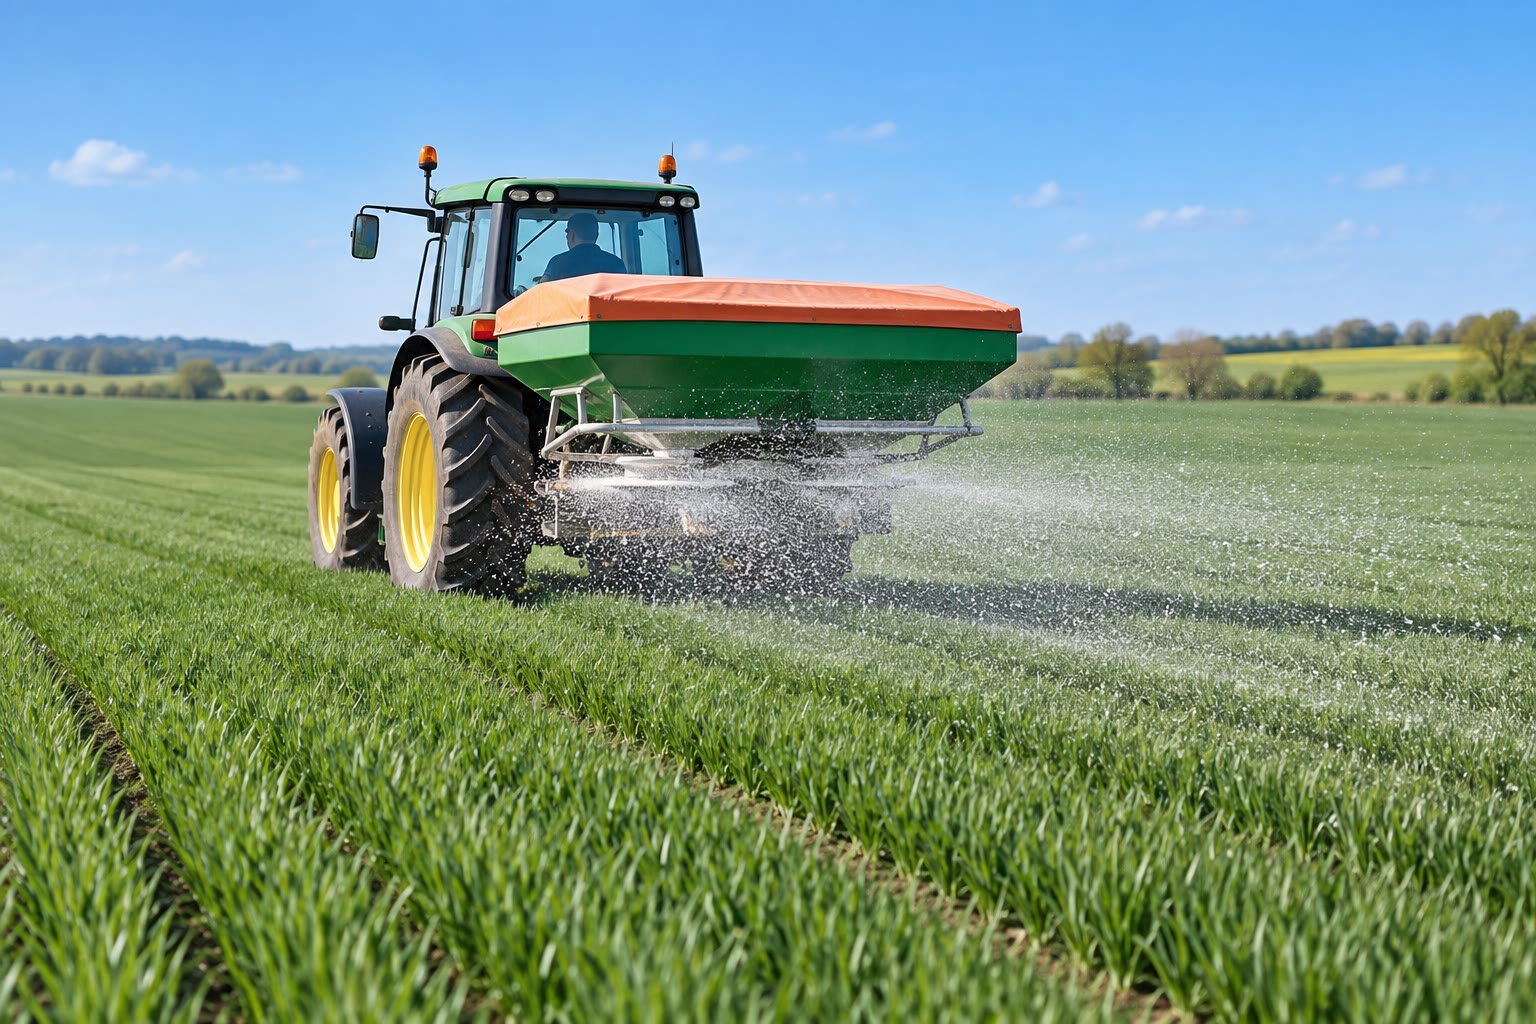
\includegraphics[width=0.55\linewidth]{images/book2/ai/b1-27-fertiliser-field.jpg}

{\small गेहूँ के खेत में नाइट्रोजन उर्वरक का छिड़काव। इसका अधिकांश भाग
हेबर--बॉश प्रक्रम द्वारा वायु के नाइट्रोजन से बनाया गया था।}
\end{omfigure}

\section{समूह 13: बोरॉन और ऐलुमिनियम}

बोरॉन एक \omterm{def:b1:periodicity:metalloid}{उपधातु} है जो अपूर्ण अष्टक वाले सहसंयोजी यौगिक बनाता है:
\ce{BF3} और बोरिक अम्ल \ce{B(OH)3} में बोरॉन के छह \omterm{def:b1:quantum-numbers:configuration}{संयोजकता
इलेक्ट्रॉन} होते हैं और वह \omterm{def:b1:lewis-resonance-vsepr:lewis-acid}{लुइस अम्ल} की तरह कार्य करता है (\cref{ch:b1:lewis-resonance-vsepr})।
बोरिक अम्ल प्रोटॉन खोकर नहीं, बल्कि एक हाइड्रॉक्साइड आयन ग्रहण करके
\omterm{def:b1:predominant-reaction:strong-acid}{दुर्बल अम्ल} है, \ce{B(OH)3 + 2H2O <=> B(OH)4- + H3O+}। बोरैक्स, एक सोडियम
बोरेट, काँच और अपमार्जकों में प्रयुक्त होता है।

\begin{definition}[ऑक्सोअम्ल]\label{def:b1:p-block-13-15:oxoacid}
\emph{ऑक्सोअम्ल}\index{ऑक्सोअम्ल} ऐसा अम्ल है जिसके अम्लीय हाइड्रोजन
परमाणु ऐसे ऑक्सीजन परमाणुओं से आबंधित हैं जो एक \omterm{def:b1:complexation:complex}{केंद्रीय परमाणु} से आबंधित हैं:
\ce{B(OH)3}, \ce{H2CO3}, \ce{HNO3} (\ce{HO-NO2}), \ce{H3PO4}
(\ce{(HO)3PO}), \ce{H2SO4}। \omterm{def:b1:complexation:complex}{केंद्रीय परमाणु} के चारों ओर हाइड्रोजन-रहित ऑक्सीजन
परमाणु जितने अधिक, अम्ल उतना ही प्रबल।
\end{definition}

बोरॉन के नीचे ऐलुमिनियम एक धातु है, पर उसका छोटा, उच्च आवेशित आयन
उसे \omterm{def:b1:s-block:oxide-character}{उभयधर्मी ऑक्साइड} और हाइड्रॉक्साइड देता है (\cref{sec:b1:precipitation:amphoteric})।
उसका अयस्क बॉक्साइट है, जो लौह ऑक्साइडों और सिलिका के साथ ऐलुमिनियम हाइड्रॉक्साइडों का
मिश्रण है; 2025 में संसार ने लगभग 44 करोड़ टन बॉक्साइट खोदा और
उससे लगभग 15 करोड़ टन ऐलुमिना परिष्कृत किया।
% ledger: usgs:bauxite-world-2025, usgs:alumina-world-2025

\begin{proposition}[बायर प्रक्रम]\label{prop:b1:p-block-13-15:bayer}
गरम सांद्र सोडियम हाइड्रॉक्साइड बॉक्साइट के ऐलुमिनियम को
\ce{Al(OH)4-} के रूप में घोल देता है और लौह ऑक्साइडों (लाल पंक) को छोड़ देता है; छने हुए विलयन को
ठंडा करने और उसमें बीज डालने से शुद्ध \ce{Al(OH)3} अवक्षेपित होता है, जिसे निस्तापित करके ऐलुमिना बनाया जाता है,
\ce{2Al(OH)3 -> Al2O3 + 3H2O}।
\end{proposition}

\begin{proof}
\qty{25}{\celsius} पर \ce{Al(OH)3(s) + OH- <=> Al(OH)4-} का $K = 10^{-1.23}$ है
(\cref{ch:b1:precipitation}): ऊँचे \ce{[OH-]} पर
ऐलुमिनियम विलयन में रहता है, जबकि आयरन(III) हाइड्रॉक्साइड, जो उभयधर्मी नहीं है,
ठोस बना रहता है (\cref{exo:b1:precipitation:12})। तनुकरण और ठंडा करना
\ce{[OH-]} को घटाते हैं और भागफल को इस प्रकार खिसकाते हैं कि उत्क्रम अभिक्रिया के लिए
$Q > K$ हो जाए: हाइड्रॉक्साइड अवक्षेपित होता है। निस्तापन जल हटा देता है।
\end{proof}

फिर ऐलुमिना को गलित क्रायोलाइट में विद्युत-अपघटन द्वारा ऐलुमिनियम में अपचित किया जाता है,
एक उद्योग जिसका अध्ययन द्वितीय वर्ष के खंड में है।

\begin{omfigure}
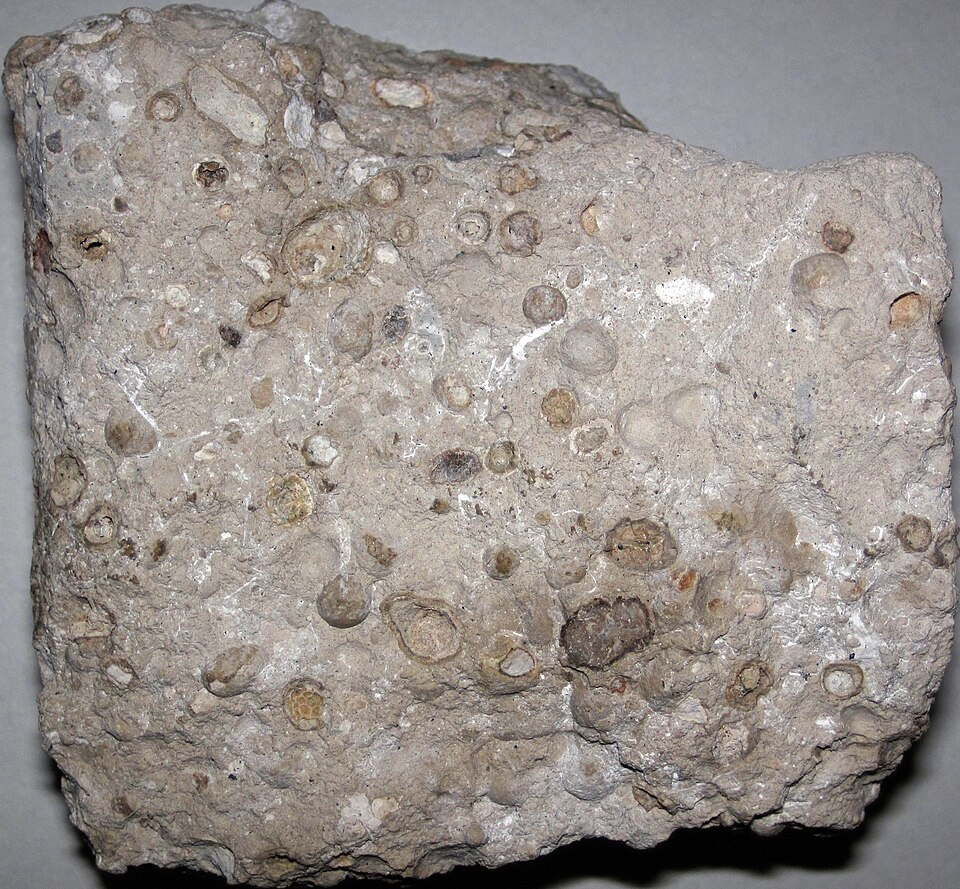
\includegraphics[height=3.6cm]{images/book2/bauxite.jpg}\hspace{0.4em}%
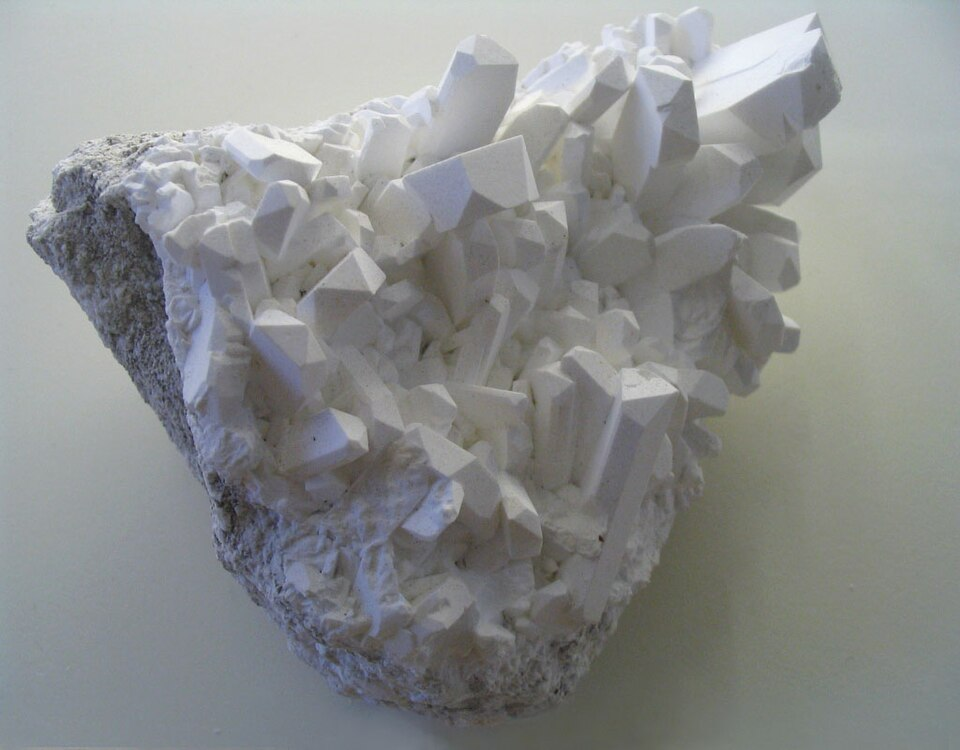
\includegraphics[height=3.6cm]{images/book2/borax.jpg}\hspace{0.4em}%
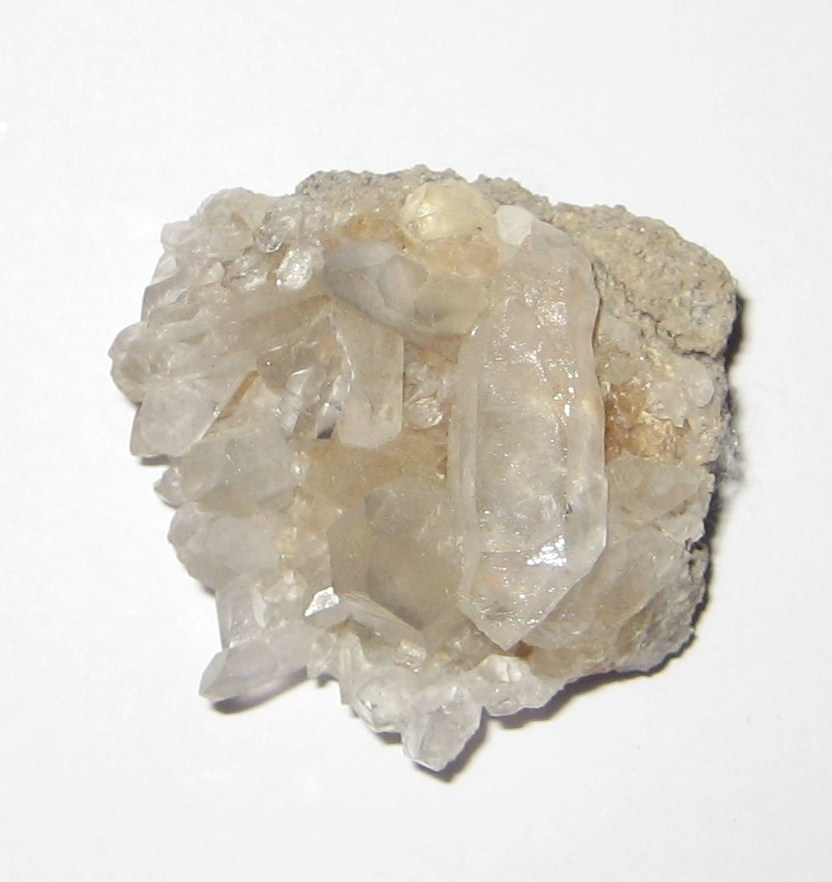
\includegraphics[height=3.6cm]{images/book2/quartz.jpg}\hspace{0.4em}%
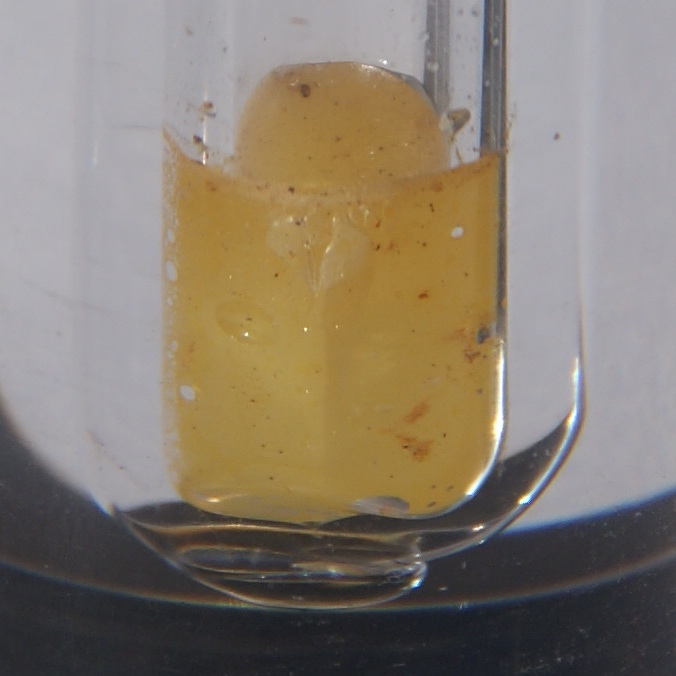
\includegraphics[height=3.6cm]{images/book2/white-phosphorus.jpg}

{\small बाएँ से दाएँ: पिसोलिटिक बॉक्साइट (जेम्स सेंट जॉन, CC BY 2.0);
बोरैक्स के \omterm{def:b1:crystals-metals:crystal}{क्रिस्टल} (अराम दुल्यान, सार्वजनिक अधिकार-क्षेत्र); क्वार्ट्ज़ \omterm{def:b1:crystals-metals:crystal}{क्रिस्टलों} का एक गुच्छ,
\ce{SiO2} (स्टेफ़नी क्लिफ़र्ड, CC BY 2.0); श्वेत फ़ॉस्फ़ोरस, थोड़े
लाल फ़ॉस्फ़ोरस के साथ, जल के नीचे रखा गया क्योंकि वह वायु में प्रज्वलित हो जाता है (हाई-रेज़ इमेजेज़
ऑफ़ केमिकल एलिमेंट्स, CC BY 3.0)। सभी विकिमीडिया कॉमन्स।}
\end{omfigure}

\section{समूह 14: कार्बन और सिलिकॉन}

कार्बन और सिलिकॉन दोनों चार आबंध बनाते हैं, पर भिन्न ढंग से। कार्बन
प्रबल द्वि-आबंध बनाता है: \ce{CO2} एक अणु है, \ce{O=C=O}, एक गैस। सिलिकॉन
शायद ही ऐसा करता है: \ce{SiO2} उन \ce{SiO4} चतुष्फलकों का सहसंयोजी जाल है
जो अपने सभी कोने साझा करते हैं, एक कठोर ठोस, क्वार्ट्ज़ (\cref{ch:b1:crystals-ionic-covalent})।
कार्बन डाइऑक्साइड एक \omterm{def:b1:s-block:oxide-character}{अम्लीय ऑक्साइड} है, जो कार्बोनिक अम्ल, हाइड्रोजनकार्बोनेट
और कार्बोनेट देता है (\cref{ch:b1:predominant-reaction}); सिलिका भी एक \omterm{def:b1:s-block:oxide-character}{अम्लीय
ऑक्साइड} है, जिस पर गलित क्षार आक्रमण करके सिलिकेट देता है।

\begin{proposition}[सिलिकेट इकाइयाँ]\label{prop:b1:p-block-13-15:silicate-units}
सिलिकेट \ce{SiO4} चतुष्फलकों से बने होते हैं; अन्य चतुष्फलकों के साथ साझा
कोनों की संख्या ऋणायन का सूत्र निर्धारित करती है: कोई नहीं, \ce{SiO4^4-}
(पृथक चतुष्फलक); दो, शृंखलाएँ $(\ce{SiO3})_n^{2n-}$; तीन, परतें
$(\ce{Si2O5})_n^{2n-}$; चार, उदासीन ढाँचा \ce{SiO2}।
\end{proposition}

\begin{proof}
साझा ऑक्सीजन आधा-आधा दोनों चतुष्फलकों का होता है। $k$ कोने साझा करने वाला चतुष्फलक
$4 - k$ ऑक्सीजन परमाणुओं का पूरा स्वामी है और $k$ का आधा: प्रति सिलिकॉन $4 -
k/2$ ऑक्सीजन। हर असाझा ऑक्सीजन पर आवेश $-1$ होता है (उसका
एक आबंध है), हर साझा ऑक्सीजन पर कोई नहीं: प्रति सिलिकॉन आवेश
$-(4 - k)$ है। $k = 0$: \ce{SiO4^4-}; $k = 2$: प्रति सिलिकॉन \ce{SiO3^2-};
$k = 3$: \ce{SiO_{2.5}^-}, अर्थात् \ce{Si2O5^2-}; $k = 4$: \ce{SiO2}।
\end{proof}

\begin{omfigure}
\begin{tikzpicture}[font=\small, line join=round]
  % one SiO4 tetrahedron in perspective
  \begin{scope}
    \coordinate (t) at (0,1.2); \coordinate (a) at (-1.0,-0.5);
    \coordinate (b) at (1.0,-0.5); \coordinate (c) at (0.25,0.05);
    \draw[thick, omDef] (t) -- (a) -- (b) -- cycle; \draw[thick, omDef] (t) -- (b);
    \draw[dashed, omDef] (a) -- (c) -- (b) (t) -- (c);
    \foreach \p in {t,a,b,c} \shade[ball color=red!60] (\p) circle (0.16);
    \shade[ball color=gray!40] (0.06,0.18) circle (0.11);
    \node at (0,-1.2) {\ce{SiO4^4-}: एक चतुष्फलक};
  \end{scope}
  % a chain of tetrahedra seen from above
  \begin{scope}[xshift=3.6cm]
    \foreach \i in {0,1,2,3} {
      \draw[thick, omDef, fill=omDef!10] (\i*1.1,0) -- (\i*1.1+0.55,0.95) -- (\i*1.1+1.1,0) -- cycle;
      \shade[ball color=red!60] (\i*1.1+0.55,0.95) circle (0.12);
      \shade[ball color=red!60] (\i*1.1+0.55,0.32) circle (0.10);
    }
    \foreach \i in {0,1,2,3,4} \shade[ball color=red!60] (\i*1.1,0) circle (0.12);
    \node[align=center] at (2.2,-1.0) {शृंखला $(\ce{SiO3})_n^{2n-}$: हर चतुष्फलक\\ दो कोने साझा करता है (ऊपर से देखा गया)};
  \end{scope}
\end{tikzpicture}

{\small सिलिकेट इकाइयाँ: एक पृथक \ce{SiO4} चतुष्फलक (सिलिकॉन धूसर,
ऑक्सीजन लाल), और एक शृंखला जिसमें हर चतुष्फलक दो ऑक्सीजन
परमाणु अपने पड़ोसियों के साथ साझा करता है। परतें (तीन साझा कोने) अभ्रक और
मृत्तिकाएँ बनाती हैं; ढाँचा (चार) क्वार्ट्ज़ बनाता है।}
\end{omfigure}

\begin{definition}[अक्रिय युग्म प्रभाव]\label{def:b1:p-block-13-15:inert-pair}
\emph{अक्रिय युग्म प्रभाव}\index{अक्रिय युग्म प्रभाव} \omterm{def:b1:periodicity:table}{समूह} 13 से 15 में नीचे
जाने पर, समूह की उच्चतम ऑक्सीकरण अवस्था से दो कम वाली अवस्था का बढ़ता हुआ
स्थायित्व है: (III) के बजाय थैलियम(I), (IV) के बजाय लेड(II),
(V) के बजाय बिस्मथ(III)। भारी तत्त्वों का \textit{ns}$^2$ युग्म
दृढ़ता से बँधा रहता है और आबंधन में बहुत कम भाग लेता है।
\end{definition}

यह प्रभाव समझाता है कि लेड(IV) ऑक्साइड प्रबल \omterm{def:b1:nernst:couple}{ऑक्सीकारक} क्यों है
($E^\circ(\ce{PbO2}/\ce{Pb^2+}) = 1.46$~V, \cref{ch:b1:nernst}), जबकि
कार्बन(IV) और सिलिकॉन(IV) अपने तत्त्वों की स्थायी अवस्थाएँ हैं।

\section{समूह 15: नाइट्रोजन}

\begin{proposition}[नाइट्रोजन की सीढ़ी]\label{prop:b1:p-block-13-15:nitrogen-ladder}
नाइट्रोजन $-3$ से $+5$ तक हर \omterm{def:b1:nernst:oxidation-number}{ऑक्सीकरण संख्या} लेता है: \ce{NH3} और
\ce{NH4+} ($-$III), \ce{N2H4} ($-$II), \ce{NH2OH} ($-$I), \ce{N2} (0),
\ce{N2O} ($+$I), \ce{NO} ($+$II), \ce{HNO2} और \ce{NO2-} ($+$III),
\ce{NO2} ($+$IV), \ce{HNO3} और \ce{NO3-} ($+$V)।
\end{proposition}

\begin{proof}
H को $+$I और O को $-$II लेकर, हर सूत्र पर \cref{prop:b1:nernst:on-rules} के नियम
लागू कीजिए: \ce{N2H4} में $2x + 4 = 0$; \ce{NO2-} में $x - 4 =
-1$; इत्यादि।
\end{proof}

\begin{definition}[नाइट्रोजन स्थिरीकरण]\label{def:b1:p-block-13-15:nitrogen-fixation}
\emph{नाइट्रोजन स्थिरीकरण}\index{नाइट्रोजन स्थिरीकरण} ऐसी कोई भी प्रक्रिया है जो
वायु के डाइनाइट्रोजन को ऐसे यौगिक (अमोनिया, नाइट्रेट) में बदले
जिसका उपयोग जीव या उद्योग कर सकें: जीवाणुओं द्वारा जैविक स्थिरीकरण,
तड़ित द्वारा स्थिरीकरण, और अमोनिया का औद्योगिक संश्लेषण।
\end{definition}

हेबर--बॉश प्रक्रम लोहे के \omterm{def:b1:elementary-steps:catalyst}{उत्प्रेरक} पर नाइट्रोजन और हाइड्रोजन को संयोजित करता है,
\ce{N2 + 3H2 <=> 2NH3}। अभिक्रिया कमरे के
ताप पर अनुकूल है (\qty{25}{\celsius} पर $K = 10^{5.8}$, अमोनिया की निर्माण गिब्ज़ ऊर्जा
से), पर बहुत धीमी; \omterm{def:b1:elementary-steps:catalyst}{उत्प्रेरक} केवल गरम होने पर काम करता है, और
दर और \omterm{def:b1:extent-q-and-k:fractional-extent}{लब्धि} में सामंजस्य बिठाने वाले ताप और दाब का चयन
द्वितीय वर्ष के खंड में किया गया है। फिर अमोनिया को ओस्टवाल्ड प्रक्रम द्वारा
नाइट्रिक अम्ल में ऑक्सीकृत किया जाता है।
% ledger: dfg:NH3_g

\begin{omfigure}
\begin{tikzpicture}[font=\small, >={Stealth}, box/.style={draw, rounded corners, fill=omDef!8, align=center, minimum height=0.9cm}]
  \node[box] (air) at (0,0) {वायु\\\ce{N2}};
  \node[box] (gas) at (0,-1.6) {प्राकृतिक गैस\\\ce{H2}};
  \node[box] (hb) at (3.4,-0.8) {हेबर--बॉश\\लोहे का उत्प्रेरक};
  \node[box] (ox1) at (7.3,-0.8) {Pt--Rh जाली\\\ce{NH3} $\to$ \ce{NO}};
  \node[box] (ox2) at (11.0,-0.8) {ऑक्सीकरण\\अवशोषण\\\ce{NO} $\to$ \ce{NO2} $\to$ \ce{HNO3}};
  \draw[->, thick] (air) -- (hb);
  \draw[->, thick] (gas) -- (hb);
  \draw[->, thick] (hb) -- node[above] {\ce{NH3}} (ox1);
  \draw[->, thick] (ox1) -- node[above] {\ce{NO}} (ox2);
  \draw[->, thick] (ox2.south) -- ++(0,-0.6) node[below] {\ce{HNO3}};
  \draw[->, thick] (hb.south) -- ++(0,-0.9) node[below] {\ce{NH3} (उर्वरक)};
  \draw[->, thick] (ox2.north) -- ++(0,0.5) -| node[pos=0.25, above] {\ce{NO} पुनःचक्रित} (ox1.north);
\end{tikzpicture}

{\small वायु से नाइट्रिक अम्ल तक: अमोनिया संश्लेषण और उसके बाद
ओस्टवाल्ड प्रक्रम के तीन चरण।}
\end{omfigure}

\begin{method}[शृंखलाबद्ध औद्योगिक समीकरणों का संतुलन]\label{met:b1:p-block-13-15:ostwald-balance}
\begin{enumerate}
  \item हर चरण संतुलित कीजिए: (1) \ce{4NH3 + 5O2 -> 4NO + 6H2O};
        (2) \ce{2NO + O2 -> 2NO2}; (3) \ce{3NO2 + H2O -> 2HNO3 + NO}।
  \item चरणों को इस प्रकार गुणा कीजिए कि बना हर मध्यवर्ती खप जाए
        (चरण 3 का \ce{NO} चरण 2 में लौटता है)।
  \item जोड़िए: NO के पूर्ण पुनःचक्रण के साथ समग्र समीकरण
        \ce{NH3 + 2O2 -> HNO3 + H2O} है, प्रति अमोनिया एक नाइट्रिक अम्ल।
  \item द्रव्यमान संतुलनों के लिए समग्र समीकरण का, और हर रिऐक्टर के
        अभिकल्पन के लिए चरणों का उपयोग कीजिए।
\end{enumerate}
\end{method}

\begin{history}[फ़्रिट्ज़ हेबर]
\begin{minipage}[t]{0.18\linewidth}\vspace{0pt}
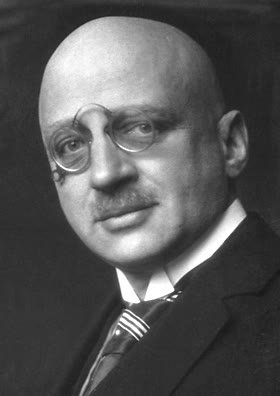
\includegraphics[width=\linewidth]{images/book2/haber.jpg}
\end{minipage}\hfill
\begin{minipage}[t]{0.78\linewidth}\vspace{0pt}
फ़्रिट्ज़ हेबर ने दिखाया कि अमोनिया नाइट्रोजन और हाइड्रोजन से
दाब में किसी \omterm{def:b1:elementary-steps:catalyst}{उत्प्रेरक} पर बनाई जा सकती है; कार्ल बॉश ने प्रयोगशाला की अभिक्रिया को
एक औद्योगिक प्रक्रम में बदल दिया। हेबर को 1918 का रसायन का नोबेल पुरस्कार
मिला। उसी व्यक्ति ने प्रथम विश्वयुद्ध में क्लोरीन के एक हथियार के रूप में पहले
बड़े पैमाने के उपयोग का निर्देशन किया: जो रसायन आधी मानवता को भोजन देता है
और जो रसायन मारता है, उन्हें रसायनज्ञों के चयन अलग करते हैं।
(छायाचित्र: नोबेल फ़ाउंडेशन, 1919 में प्रकाशित, सार्वजनिक अधिकार-क्षेत्र,
विकिमीडिया कॉमन्स।)
\end{minipage}
\end{history}

\section{फ़ॉस्फ़ोरस और समूहों में नीचे की प्रवृत्तियाँ}

नाइट्रोजन के नीचे फ़ॉस्फ़ोरस \ce{P#P} त्रि-आबंध नहीं बनाता: श्वेत
फ़ॉस्फ़ोरस \ce{P4} चतुष्फलकों से बना है, जो तनावयुक्त और क्रियाशील हैं (वह
वायु में प्रज्वलित हो जाता है और जल के नीचे रखा जाता है); लाल फ़ॉस्फ़ोरस एक बहुलक है,
जो कहीं कम क्रियाशील है। फ़ॉस्फ़ोरस को जलाने से \ce{P4O10} मिलता है, जो
सामान्य ऑक्साइडों में सबसे अम्लीय है, और जल के साथ फ़ॉस्फ़ोरिक अम्ल देता है,
$\mathrm{p}K_a$ 2.15, 7.21, 12.34 (\cref{ch:b1:predominant-reaction})।
फ़ॉस्फ़ेट चट्टान, जो 2025 में लगभग 25 करोड़ टन खोदी गई, को
सल्फ़्यूरिक अम्ल फ़ॉस्फ़ेट उर्वरकों में बदल देता है।
% ledger: usgs:phosphate-world-2025

हर समूह में नीचे जाने पर तत्त्व अधिक धात्विक होते जाते हैं (बोरॉन से थैलियम,
कार्बन से लेड, नाइट्रोजन से बिस्मथ), उनके ऑक्साइड अधिक क्षारकीय, और
निम्नतर ऑक्सीकरण अवस्थाएँ अधिक स्थायी: \omterm{def:b1:p-block-13-15:inert-pair}{अक्रिय युग्म प्रभाव}। किसी
\omterm{def:b1:periodicity:table}{आवर्त} में आगे बढ़ने पर ऑक्साइड अधिक अम्लीय होते जाते हैं, क्षारकीय \ce{Na2O} से फ़ॉस्फ़ोरस और सल्फ़र के
\omterm{def:b1:s-block:oxide-character}{अम्लीय ऑक्साइडों} तक।

\section{अभ्यास}

\begin{exercise}[$\star$]\label{exo:b1:p-block-13-15:1}
\ce{NH4NO3} (दोनों परमाणु), \ce{N2O5}, \ce{HNO2}, \ce{N2H4} और \ce{Mg3N2} में
नाइट्रोजन की \omterm{def:b1:nernst:oxidation-number}{ऑक्सीकरण संख्या} बताइए।
\end{exercise}

\begin{exercise}[$\star$]\label{exo:b1:p-block-13-15:2}
\ce{BF3}, \ce{NH3} और योगज
\ce{F3B-NH3} की \omterm{def:b1:lewis-resonance-vsepr:lewis}{लुइस संरचनाएँ} खींचिए; \omterm{def:b1:lewis-resonance-vsepr:lewis-acid}{लुइस अम्ल} और क्षारक पहचानिए।
\end{exercise}

\begin{exercise}[$\star$]\label{exo:b1:p-block-13-15:3}
सोडियम हाइड्रॉक्साइड के साथ \ce{CO2}, \ce{SiO2} (गलित) और \ce{P4O10} की, और
एक अम्ल तथा एक क्षारक के साथ \ce{Al2O3} की अभिक्रियाएँ लिखिए।
\end{exercise}

\begin{exercise}[$\star$]\label{exo:b1:p-block-13-15:4}
\qty{25}{\celsius} पर \ce{N2 + 3H2 <=> 2NH3} का साम्य स्थिरांक
$\Delta_f G^\circ(\ce{NH3}) =
\qty{-16.45}{kJ/mol}$ से परिकलित कीजिए।
\end{exercise}

\begin{exercise}[$\star\star$]\label{exo:b1:p-block-13-15:5}
\cref{prop:b1:p-block-13-15:silicate-units} की गणना का उपयोग करके,
दो-दो कोने साझा करने वाले छह चतुष्फलकों के वलय (जैसे बेरिल में) का
और ऐसी द्वि-शृंखला का सूत्र बताइए जिसमें आधे चतुष्फलक दो कोने और
आधे तीन कोने साझा करते हैं।
\end{exercise}

\begin{exercise}[$\star\star$]\label{exo:b1:p-block-13-15:6}
द्रव्यमान से \qty{55}{\percent} \ce{Al(OH)3} युक्त एक टन बॉक्साइट से
\qty{92}{\percent} पुनःप्राप्ति के साथ प्राप्त ऐलुमिना का द्रव्यमान
परिकलित कीजिए।
\end{exercise}

\begin{exercise}[$\star\star$]\label{exo:b1:p-block-13-15:7}
दिखाइए कि बोरिक अम्ल \omterm{def:b1:predominant-reaction:bronsted}{ब्रॉन्स्टेड अम्ल} के बजाय \omterm{def:b1:lewis-resonance-vsepr:lewis-acid}{लुइस अम्ल} है, और
समझाइए कि फिर भी उसका विलयन अम्लीय क्यों है।
\end{exercise}

\begin{exercise}[$\star\star$]\label{exo:b1:p-block-13-15:8}
\omterm{def:b1:nernst:oxidation-number}{ऑक्सीकरण संख्याओं} से अमोनिया के \ce{NO} तक ऑक्सीकरण को संतुलित कीजिए और
प्रति \ce{NH3} विनिमित इलेक्ट्रॉनों की संख्या बताइए।
\end{exercise}

\begin{exercise}[$\star\star$]\label{exo:b1:p-block-13-15:9}
अमोनियम नाइट्रेट अमोनिया और नाइट्रिक अम्ल से बनाया जाता है। अभिक्रिया लिखिए,
और प्रति टन अमोनियम नाइट्रेट आवश्यक अमोनिया का द्रव्यमान (नाइट्रिक अम्ल के लिए और
उदासीनीकरण के लिए, दोनों) परिकलित कीजिए।
\end{exercise}

\begin{exercise}[$\star\star\star$]\label{exo:b1:p-block-13-15:10}
द्वितीय-आवर्त और तृतीय-आवर्त परमाणुओं के बीच $\pi$ आबंधों की प्रबलता का उपयोग करके
समझाइए कि नाइट्रोजन द्विपरमाणुक गैस और फ़ॉस्फ़ोरस \ce{P4}
अणुओं का ठोस क्यों है, और कार्बन डाइऑक्साइड गैस और सिलिका ठोस क्यों है।
\end{exercise}

\begin{exercise}[$\star\star\star$]\label{exo:b1:p-block-13-15:11}
\omterm{def:b1:nernst:electrode-potential}{मानक विभवों} से दिखाइए कि लेड(IV) ऑक्साइड अम्ल में क्लोराइड
आयनों को क्लोरीन में ऑक्सीकृत करता है, जबकि सिलिकॉन(IV) ऑक्साइड ऐसा कुछ
नहीं करता। इसे \omterm{def:b1:p-block-13-15:inert-pair}{अक्रिय युग्म प्रभाव} से जोड़िए।
\end{exercise}

\begin{exercise}[$\star\star\star$]\label{exo:b1:p-block-13-15:12}
संसार ने 2025 में अमोनिया के रूप में लगभग 16 करोड़ टन नाइट्रोजन बनाया।
यह अमोनिया का कितना द्रव्यमान है, और उसमें हाइड्रोजन का कितना द्रव्यमान था?
वह हाइड्रोजन मुख्यतः कहाँ से आता है?
\end{exercise}

\section{समस्या: वायु से उर्वरक तक}

\begin{problem}[{सप्ताहांत समस्या --- नाइट्रोजन त्रि-आबंध, अमोनिया
संश्लेषण, नाइट्रिक अम्ल निर्माण के तीन चरण, अमोनियम नाइट्रेट,
और एक टन अमोनिया से प्राप्त हो सकने वाले नाइट्रिक अम्ल का द्रव्यमान}]
\label{pb:b1:p-block-13-15:1}
एक उर्वरक संयंत्र अमोनिया को नाइट्रिक अम्ल और अमोनियम
नाइट्रेट में बदलता है। मोलर द्रव्यमान (\unit{g/mol}): \ce{N2} 28.0, \ce{H2} 2.0, \ce{NH3}
17.0, \ce{HNO3} 63.0, \ce{NH4NO3} 80.0, \ce{O2} 32.0;
\qty{25}{\celsius} पर $\Delta_f G^\circ(\ce{NH3(g)}) = \qty{-16.45}{kJ/mol}$।

\medskip
\noindent\textbf{भाग I --- नाइट्रोजन।}
\begin{enumerate}
  \item \ce{N2} की \omterm{def:b1:lewis-resonance-vsepr:lewis}{लुइस संरचना} खींचिए और बताइए कि वह अनभिक्रियाशील क्यों है।
  \item \ce{N2}, \ce{NH3}, \ce{NO},
        \ce{NO2}, \ce{HNO3} और \ce{NH4NO3} में N की \omterm{def:b1:nernst:oxidation-number}{ऑक्सीकरण संख्या} बताइए।
  \item नाइट्रोजन के स्थिरीकरण के तीन प्राकृतिक या औद्योगिक ढंग बताइए।
  \item पौधे \ce{N2} का सीधे उपयोग क्यों नहीं कर पाते?
  \item अमोनिया के संश्लेषण में कौन-सा तत्त्व ऑक्सीकृत होता है और कौन-सा अपचित?
  \item अमोनिया का संश्लेषण लिखिए।
\end{enumerate}

\medskip
\noindent\textbf{भाग II --- अमोनिया।}
\begin{enumerate}[resume]
  \item \qty{25}{\celsius} पर संश्लेषण का साम्य स्थिरांक परिकलित
        कीजिए।
  \item फिर भी संश्लेषण गरम अवस्था में, \omterm{def:b1:elementary-steps:catalyst}{उत्प्रेरक} पर, क्यों चलाया जाता है?
  \item एक टन अमोनिया के लिए \ce{N2} और \ce{H2} के द्रव्यमान परिकलित
        कीजिए।
  \item वायु का कितना आयतन (आयतन से \qty{78}{\percent} \ce{N2}, आदर्श
        गैस, \qty{25}{\celsius}, \qty{1}{bar}) उस नाइट्रोजन को समाहित करता है?
  \item हाइड्रोजन कहाँ से आता है?
  \item कुछ देशों में अमोनिया स्वयं उर्वरक के रूप में क्यों प्रयुक्त होती है, और
        उसे प्रायः पहले रूपांतरित क्यों किया जाता है?
\end{enumerate}

\medskip
\noindent\textbf{भाग III --- नाइट्रिक अम्ल।}
\begin{enumerate}[resume]
  \item \omterm{def:b1:nernst:oxidation-number}{ऑक्सीकरण संख्याओं} से चरण 1, \ce{NH3 + O2 -> NO + H2O}, संतुलित कीजिए। % ce-unbalanced-ok
  \item चरण 2, \ce{NO + O2 -> NO2}, संतुलित कीजिए। % ce-unbalanced-ok
  \item चरण 3, \ce{NO2 + H2O -> HNO3 + NO}, संतुलित कीजिए। यह किस प्रकार की अपचयोपचय % ce-unbalanced-ok
        अभिक्रिया है?
  \item NO के पूर्ण पुनःचक्रण के साथ चरणों को संयोजित करके समग्र
        समीकरण बनाइए।
  \item प्रति टन अमोनिया खपी ऑक्सीजन का द्रव्यमान परिकलित कीजिए।
  \item चरण 1 में प्लैटिनम--रोडियम जाली क्यों प्रयुक्त होती है?
\end{enumerate}

\medskip
\noindent\textbf{भाग IV --- अमोनियम नाइट्रेट और द्रव्यमान संतुलन।}
\begin{enumerate}[resume]
  \item अमोनियम नाइट्रेट का बनना लिखिए।
  \item केवल अमोनियम नाइट्रेट बनाने के लिए अमोनिया का कितना अंश नाइट्रिक अम्ल में
        बदलना होगा?
  \item इस प्रकार बाँटी गई एक टन अमोनिया से अमोनियम नाइट्रेट का द्रव्यमान
        परिकलित कीजिए।
  \item अमोनियम नाइट्रेट में नाइट्रोजन का प्रतिशत कितना है?
  \item अमोनियम नाइट्रेट को ईंधनों और ऊष्मा से दूर क्यों रखना चाहिए?
  \item एक टन अमोनिया (पूर्ण रूपांतरण) से प्राप्त हो सकने वाले नाइट्रिक अम्ल का द्रव्यमान
        परिकलित कीजिए।
\end{enumerate}
\end{problem}
